\section{Motivation and Background}

\subsection {Asynchronous Programming in Representative NFs}
\label{sec:bro}


\begin{comment}
\begin{figure}[!t]
\centering
\begin{lstlisting}[style=CStyle]
void Hash::Finalize() {
	...
  // Generate file_hash event if a transmitted file is
  // detected.
	mgr.QueueEvent(file_hash, vl);
}
EventHandler::Call(val_list* vl, bool no_remote) {
  // file_hash EventHandler
  ...
  // Eventually query local store.
  bro_broker::StoreQueryCallback* cb;
  ...
  handle->store->lookup(..., cb);
}
StoreQueryCallback::Result(RecordVal* result) {
  // If file hash is in local store, log the detected
  // malware and quit.
  ...
  // If file hash is not in local store, eventually
  // query DNS.
  dns_mgr->AsyncLookupNameText(..., new LookupHostCallback(...));
}
Trigger::Timeout(){
  ...
  // Log a malware-detection error in case local
  // database timeout.
}
LookupHostCallback::Resolved(TableVal* addrs) {
  ...
  // If file hash is in MHR service, log the detected
  // malware. Otherwise quit.
}
LookupHostCallback::Timeout() {
  ...
  // Log a malware-detection error in case DNS
  // query timeouts.
}
\end{lstlisting}
\caption{Malware detection in Bro.}
\label{fig:code-sample}
\end{figure}
\end{comment}

\begin{figure}[!h]
\centering
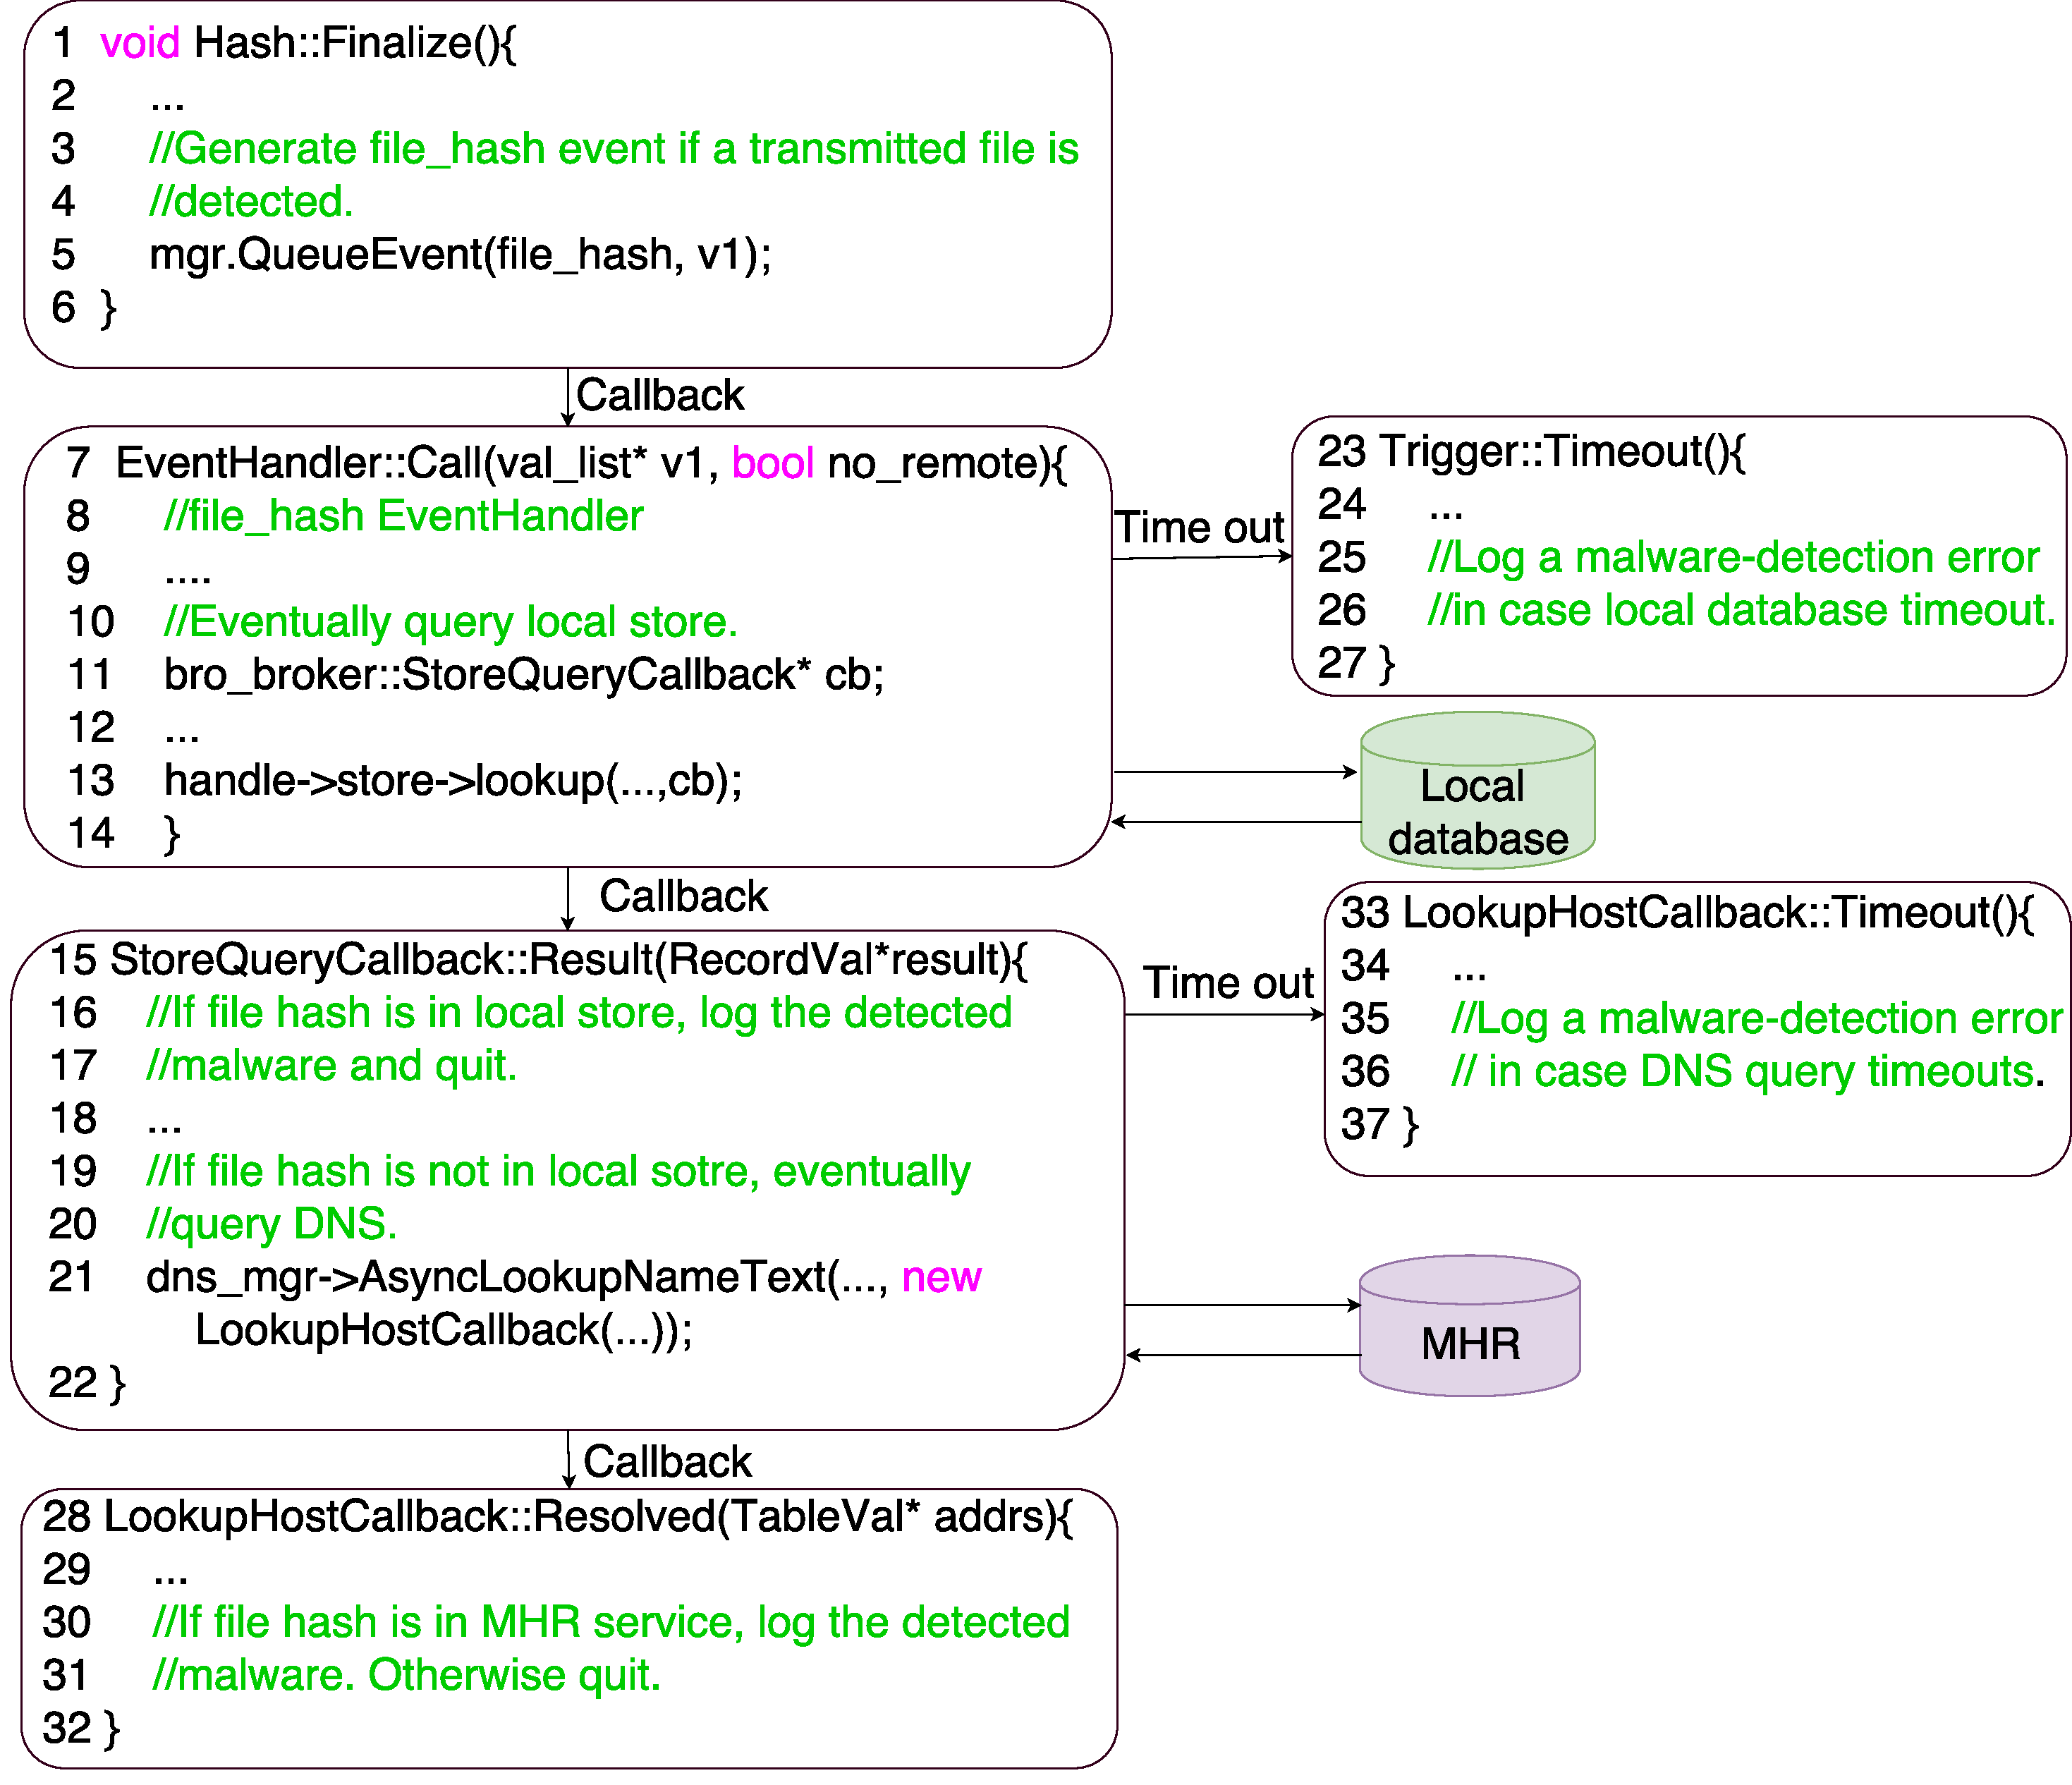
\includegraphics[width=\columnwidth]{chap-netstar/figure/ids_process_loop.pdf}
\caption{Malware detection in Bro.}
\label{fig:code-sample}
\end{figure}

\noindent\textbf{Bro.} We use a concrete example, malware detection in Bro IDS \cite{bro}, to demonstrate how asynchronous callbacks are used to program NFs. Bro can be configured to detect malware contained in a transmitted file as follows. % we can write a script to detect whether the transmitted file contains a malware. The detection method is to calculate a SHA1 hash over the content of the file and searching the calculated hash value over a set of pre-calculated malware hash values.
 A local database server %in Bro
 stores hash values of commonly-seen malware. For each TCP connection that goes through, Bro reconstructs its byte stream. % and analyzes the content of the byte stream.
 If a transmitted file is detected within the byte stream, Bro computes a SHA1 hash value over the file content, and queries the local database to obtain a quick response whether the hash value matches any malware's. In case of no hit in the local database, Bro can turn to the more complete and up-to-date Malware Hash Registry (MHR) \cite{MHR}, which provides a special DNS service: Bro can send a DNS request carrying the file hash to MHR, and the MHR responds whether there is a match with any of the malware hash values it has. If either of the two queries detects some malware, Bro raises an alarm in the log file.

The C++ code covering the execution path of the malware detection steps is given in Fig.~\ref{fig:code-sample}, as extracted from Bro version 2.5-359. In the packet processing loop of Bro, after a transmitted file is detected, \lstinline[style=InlineStyle]{Hash::Finalize()} is called to calculate the file's hash value and post a \lstinline[style=InlineStyle]{file_hash} event to Bro's event engine. Bro handles the event in the callback \lstinline[style=InlineStyle]{EventHandler::Call}, by performing an asynchronous query to the local database (lines 11,13). The response of the database query is handled by the callback \lstinline[style=InlineStyle]{StoreQueryCallback::Result}: if the file hash is not found in the local database, Bro performs another asynchronous query to the MHR (line 21). The DNS response is handled by a second callback, \lstinline[style=InlineStyle]{LookupHostCallback::Resolved}, which logs the detection of a piece of malware if the DNS response indicates so. %file hash is presented in MHR.
 Since any of the database and MHR queries may fail, two additional callbacks, \lstinline[style=InlineStyle]{Trigger::Timeout()} and \lstinline[style=InlineStyle]{LookupHostCallback::Timeout()}, are registered to handle the database and MHR query timeout error, respectively.

%The code in Fig.~\ref{fig:code-sample} is fully asynchronous and achieves good performance
The code excerpt highlights the following disadvantages in callback-based asynchronous programming:
(1) The asynchronous code is more complex to implement as compared to a synchronous program. For instance, if \lstinline[style=InlineStyle]{StoreQueryCallback::Result} is to be implemented in a synchronous fashion, the programmer can directly proceed to handle the DNS response or the timeout event after calling a blocking DNS query function, without the need for saving the context information (omitted from line 21) and defining two extra callback functions elsewhere (lines 28 and 33). %\chuan{correct the line numbers}.
(2) Omitted in line 21, saving and retrieving context information can be quite troublesome, as Bro relies on reference counting to keep allocated objects alive, and needs to correctly increase the reference counts of all the objects that it intends to keep within the context when registering a callback.
(3) Two error handling functions are defined to handle potential errors in the two asynchronous operations. The two functions in fact implement the same logic, \ie, to log a malware detection error to the database, which are quite redundant.



%It is error-prone and tedious for an ordinary programmer to handle these complexities and repetitive code. Bro resorts to a powerful script engine \cite{}, \eg, all the concrete implementation of the callbacks (lines 7, 15, 23, 28, 33 in Fig.~\ref{fig:code-sample}) is automatically generated by the script engine. However, it is even harder to implement this script engine, % than all these asynchronous callbacks and it
% highly customized for IDS tasks. % making it hard to adapt to general-purpose dataplane processing.

%\subsection{Asynchronous Programming in Other NFs}
%\label{sec:ap_in_nf}

\noindent\textbf{HAProxy.}
%Asynchronous programming with callbacks increases the implementation complexity of NFs. %Besides the example code discussed in Sec.~\ref{sec:bro},
 We have also inspected the asynchronous program in HAProxy \cite{haproxy}, a high-speed proxy due to its completely asynchronous design. HAProxy accepts incoming user TCP connections, relays received packet contents, such as HTTP requests, to several servers (\eg, for load-balancing or connecting an internal network to the public network), and then relays the responses received from the servers back to the client.
 In order to poll a socket file descriptor to retrieve the incoming data over the TCP connection, HAProxy invokes three nested callbacks, \lstinline[style=InlineStyle]{iocb} (for accessing the socket), \lstinline[style=InlineStyle]{recv} (for receiving data from the socket) and \lstinline[style=InlineStyle]{rcv_buf} (for putting received data into buffer). These three callbacks are registered multiple times in various source files, making it hard to trace the execution flow of HAProxy without a deep inspection of the files.

%\chuan{illustrate significance of the problem: how often do the complicated callbacks happen in many representative NFs' core code?}

%\vspace{1mm}
%\noindent\textbf{S-CSCF proxy.}
%Some NFs even abandon asynchronous programming due to the implementation difficulties. An representative example is an open-source, industrial-strength S-CSCF proxy \cite{} implemented by Clearwater Project \cite{}. S-CSCF proxy needs to query an ENUM service \cite{} when processing user traffic, which is a special DNS service for translating a telephone number into an URI record that can be reached over the Internet. In Clearwater Project \cite{}, querying ENUM is implemented as a synchronous procedure: the worker thread is blocked after sending out the ENUM query and unblocked when the response is received. While this simplifies implementation, it may become a potential performance bottleneck when ENUM service is heavily queried.


%above lead to the following observation: When doing asynchronous programming in NF, it is often hard to strike a balance between good runtime performance and the simplicity of implementation. So a natural question to ask is: is there a method to achieve such a balance? We believe that the key lies in bringing advanced programming abstractions to process dataplane network flows.

\subsection{Advanced Programming Abstractions}

There is a tradeoff between simplicity and performance when implementing a NF program: On one hand, synchronous programming is easier but incurs poor performance. On the other hand, asynchronous programming using callbacks achieves much better performance at the cost of implementation complexity. Similar tradeoffs have been identified when people build server programs, such as web \cite{tornado-web-server} and database servers\cite{rethinkdb}.
The solution in those domains has been to use advanced programming abstractions, including coroutine \cite{coroutine} and future/promise \cite{claessen1999poor, li2007combining, wtf, syme2011f}, to manage the complexity of asynchronous programming while achieving good performance.

%Coroutine \cite{} is a lightweight cooperative thread. On each physical thread, there can be multiple coroutines running concurrently. A coroutine runs as if it runs in its own thread and it switches its execution to other coroutines via explicit yielding. When a coroutine needs to perform a blocking task, it saves its stack information and notifies a scheduler. The scheduler picks another coroutine to run. Only when the blocking task finishes, the coroutine that initiating the task is resumed.

%tornado web server uses coroutine. search coroutine http server
% https://rethinkdb.com/blog/improving-a-large-c-project-with-coroutines/
% and hard
Coroutine is a user-space cooperative thread: a coroutine explicitly yields its execution to other coroutines when it waits for asynchronous operations to complete. The coroutine paradigm has found its success in building asynchronous web servers \cite{tornado-web-server} and databases \cite{rethinkdb}. %\chuan{why is corouting an advanced programming abstraction? it seems just some thread execution mechanism. clarify}

With coroutine, asynchronous NFs can be very easy to implement. The NF program can be directly written as a synchronous program, which runs as multiple coroutines (threads) to handle different flows. Whenever a coroutine needs to perform an asynchronous operation, it yields its execution to other coroutines after saving its thread context, and then waits to be resumed when the asynchronous response arrives in the future.

Typical coroutine switching time can be up to hundreds of nano seconds. A typical high-performance NF needs to process hundreds of thousands of flows concurrently and millions of packets per second. The coroutine switching time may significantly slow down NF processing, which we have verified with experiments (to be presented in Sec.~\ref{sec:eval6}). % against asynchronous NFs built with future/promise abstraction.

In search for a suitable advanced programming abstraction for significantly reducing implementation complexity of asynchronous NFs, we have identified that the future/promise paradigm can be more suitable. %, if it can be properly brought in for dataplane packet processing.



%We also explore the possibility of using coroutine for NF and build a simple framework that uses coroutine to handle flow packets. For each new flow, the framework creates a new coroutine and runs the packet processing loop inside the coroutine. Whenever the NF needs to wait for asynchronous events, the coroutine simply yields its control and the NF switches to process other flows using other coroutines. We directly utilize the coroutine module in Seastar.

% However, the performance of this framework (measured in terms of number of packets processed per second) is 4-5 times slower than the framework using future/promise . Even though coroutines are user-space light-weight threads and context switches between coroutines are faster than heavy-weight kernel threads, the measured context switch time among coroutines is around 352ns. Since a single NF may processes more than 10K concurrent flows, such a context switching time is considered harmful. What's more, when using coroutines, we have lost the ability of consolidated error handling provided by future/promise.

%Therefore, compared with future/promise, coroutine is not a good choice to improve asynchronous programming for NFs.

%\subsubsection{Future/Promise.}

\subsection{Future/Promise}
\label{sec:intro-future-promise}

The future/promise abstraction is a light-weight, elegant model for asynchronous programming. It simplifies asynchronous programming by mimicking synchronous programming, and reduces redundant error handling logic by propagating exceptions.


\subsubsection{Future}
A future object is of type \lstinline[style=InlineStyle]{future<T>} and contains a value of type \lstinline[style=InlineStyle]{T}. % (the interface abstractions in this section follows those in the Seastar library).
There are two states for each future object, available and unavailable. When in the available state, a future object either contains a concrete value of type \lstinline[style=InlineStyle]{T} that can be directly used, or an exception. In the unavailable state, a future object is associated with a promise object, and can be turned into available state with the help of the associated promise object.

\subsubsection{Promise}
A promise object is of type \lstinline[style=InlineStyle]{promise<T>}, and associated with an unavailable future object. When needed (\eg, when the response of a remote query arrives, or the response times out and an exception is generated), the programmer can set either a concrete value, or an exception, to the promise object with the \lstinline[style=InlineStyle]{promise::set_value} method. The value/exception is then automatically propagated to the associated future object and turns it into the available state.

\subsubsection{Continuation Function}
The future/promise abstraction works together with continuation functions to achieve asynchronous programming. A continuation function can be appended to a future object using the \lstinline[style=InlineStyle]{future::then} method. The following code shows a continuation function appended to the \lstinline[style=InlineStyle]{fur} future object.

\begin{lstlisting}[style=InlineStyle]
future<T> fur=pr.get_future();
fur.then([captured_variables...](T t){
...
});
\end{lstlisting}

\noindent Here, the continuation is presented as a C++ lambda function \cite{cpplambda}. \lstinline[style=InlineStyle]{captured_variables} is a list of variables passed to the continuation function, which it is free to use. For instance, \lstinline[style=InlineStyle]{captured_variables} may contain a pointer to another object and the continuation function can visit this object by following the pointer. %`\lstinline[style=InlineStyle]{...}' represents the function body.
 \lstinline[style=InlineStyle]{(T t)} represents the input arguments to the continuation function.

A continuation function can be considered as a special callback function. If the future object that it is appended to is available, the continuation function is immediately invoked; otherwise, it is invoked the moment when the future object becomes available. When a continuation function is called, the future object passes its concrete value as the argument \lstinline[style=InlineStyle]{T} into the continuation function. %Therefore, the input argument type (\lstinline[style=InlineStyle]{T}) of a continuation function must be the same as the value type of the future object (\lstinline[style=InlineStyle]{future<T> fur}) that it is appended to.

\subsubsection{Transforming Future Object}
\label{sec:tranform-future-object}

%Another property of the continuation function is its ability to transform a future object.
 If a continuation function is appended to a future object \lstinline[style=InlineStyle]{a} of type \lstinline[style=InlineStyle]{future<A>}, creates a future object \lstinline[style=InlineStyle]{b} of type \lstinline[style=InlineStyle]{future<B>} and returns it as a future object \lstinline[style=InlineStyle]{transformed} of type \lstinline[style=InlineStyle]{future<B>}, then we say the future object \lstinline[style=InlineStyle]{a} is transformed into future object \lstinline[style=InlineStyle]{transformed} of type \lstinline[style=InlineStyle]{future<B>}, and \lstinline[style=InlineStyle]{transformed} only becomes available when both \lstinline[style=InlineStyle]{a} and \lstinline[style=InlineStyle]{b} are available. %; otherwise, it remains unavailable.
When \lstinline[style=InlineStyle]{transformed} becomes available, it contains the exact value of \lstinline[style=InlineStyle]{b}. % which is directly acquired from \lstinline[style=InlineStyle]{b}.

Consider the following example for asynchronous database and DNS queries:

\begin{lstlisting}[style=InlineStyle]
// Query database.
future<db_res> db_fur=_db.lookup(_hash);
future<dns_res> fur=db_fur.then([this](db_res res){
  // Do something with the database query response.
  ...
  // Query DNS.
  future<dns_res> dns_fur=_dns.lookup(domain_name);
  return dns_fur;
});
\end{lstlisting}

\noindent We first issue an asynchronous database query \lstinline[style=InlineStyle]{db.lookup()} to acquire a future object \lstinline[style=InlineStyle]{db_fur}, which contains the query response when it returns. Then, we append a continuation function to \lstinline[style=InlineStyle]{db_fur}. Inside the continuation function, an asynchronous DNS query \lstinline[style=InlineStyle]{dns.lookup()} is issued and a future object \lstinline[style=InlineStyle]{dns_fur} is obtained, which contains the DNS response once it is received. When the continuation function is done, a future object \lstinline[style=InlineStyle]{fur} is obtained, %This transforms \lstinline[style=InlineStyle]{db_fur} into \lstinline[style=InlineStyle]{fur},
 which becomes available when both \lstinline[style=InlineStyle]{db_fur} and \lstinline[style=InlineStyle]{dns_fur} are available (\ie, when both the database response and DNS response are received), and contains the received DNS response once available (passed from \lstinline[style=InlineStyle]{dns_fur}).

The returned future object can be associated with another continuation function, which further returns anther future object. In this way, we are able to chain multiple continuation functions to carry out a series of asynchronous operations. It allows us %to use the future/promise approach
to mimic synchronous programming while achieving full execution asynchrony. In the above example, the database and DNS queries appear to be sequentially executed but are in fact asynchronously performed. % as in a synchronous program.
 Also, there is no need to define callbacks elsewhere: the continuation function for handling the database response is defined right in place (in the same file where the database query is issued), but is invoked only when the database response arrives and \lstinline[style=InlineStyle]{db_fur} becomes available.

% asynchronous operation defined inside the continuation function right in place.   In particular, the database query and the DNS query are sequentially defined in the code, the continuation function is immediately appended after \lstinline[style=InlineStyle]{db_fur} is generated  continuation function is immediately appendedThe code first queries the database, wait for database response. Then it queries the DNS and wait for the DNS response.

% Since continuation function executes an asynchronous DNS query and returns the future object \lstinline[style=InlineStyle]{dns_fur} containing the DNS response, \lstinline[style=InlineStyle]{fur} represents a transformed future object containing the DNS response. \lstinline[style=InlineStyle]{fur} only becomes available when both \lstinline[style=InlineStyle]{db_fur} and \lstinline[style=InlineStyle]{dns_fur} become available. When \lstinline[style=InlineStyle]{fur} becomes available, it contains the DNS response that is queried in the continuation function.

\subsubsection{Consolidated error handling.}
\label{sec:consolidated-error-handling}
In previous example, to catch database and DNS query exceptions, we can simply append another continuation function to the future object \lstinline[style=InlineStyle]{fur} as follows:

\begin{lstlisting}[style=InlineStyle]
fur.then_wrapped([](future<dns_res> f){
  try{
    f.get();
  }
  catch(...){
    // catch whatever exceptions thrown
    // during database or DNS query
  }
});
\end{lstlisting}

\noindent Here, \lstinline[style=InlineStyle]{fur} may contain an exception that is either generated by database query or DNS query. This is due to the capability of the future/promise abstraction to propagate exceptions and bypass uncalled continuation functions in the chain, and push the exception to the final returned future object. For example, if an exception occurs during database query, \lstinline[style=InlineStyle]{db_fur} will contain the exception, and then pass it to \lstinline[style=InlineStyle]{fur} without running the continuation functions it is associtaed with; if the database query is alright but DNS query raises an exception, \lstinline[style=InlineStyle]{dns_fur} contains the exception and passes it to \lstinline[style=InlineStyle]{fur}. Finally, the exception is passed to \lstinline[style=InlineStyle]{f} when the continuation function \lstinline[style=InlineStyle]{fur.then_wrapped([](future<dns_res> f)} is invoked, thrown by \lstinline[style=InlineStyle]{f.get}, and caught inside a try-catch pair \cite{cppexception}.

Leveraging this consolidated approach to handle various errors that may occur during a series of asynchronous operations, we can effectively reduce redundant error handling code when developing asynchronous programs.

%Asynchronous operations, including logging and database writing in the previous code example, may fail and throw exceptions. Future/promise abstraction can quickly propagate the generated exception and by-pass the rest of the continuations. For instance, in the previous example, should the logging fail and throw an exception, the continuation function for database writing will be by-passed and the exception will be filled in the final future object \lstinline[style=InlineStyle]{result}.

%Leveraging this property, future/promise abstraction can implement consolidated error handling using the follow code:

%\vspace{-1mm}
%\begin{lstlisting}[style=InlineStyle]
%result.then_wrapped([](future<response> fur){
%  try{
%    fur.get();
%  }
%  catch(...){
%    // catch whatever exceptions thrown from
%    // previously-chained continuation functions
%  }
%});
%\end{lstlisting}
%\vspace{-1mm}

%Using a single try-catch pair (the default mechanism for catching exceptions in C++ \cite{}), future/promise abstraction can handle all the errors happened during database reading, logging and database writing. This can greatly reduce the number of error handling code.

\subsection{Bring Future/Promise to Dataplane}


We use the open-source Seastar \cite{seastar} library as the base for implementing our future/promise NF programming model: (i) Seastar is one of the most mature C++-based future/promise libraries, and such C++ based implementation introduces minimum runtime overhead, which is critical for high-performance NFs; (ii) Seastar is integrated with DPDK and has a built-in user-space TCP/IP stack, rendering a feasible ground for building various NFs.

However, Seastar is originally designed for creating high-performance database servers \cite{scylladb}. %Though integrated with DPDK and has a user-space TCP/IP stack,
 It only exposes a socket-like interface for interacting with application-layer payload and has no interface for directly retrieving and sending raw network packets. Yet, an interface for manipulating raw network packets is crucial for implementing L4 NFs, such as firewall, NAT and IDS.

%On the other hand, even if such an interface is added to Seastar, without another properly designed interface to process network flows, we may completely lose the advantages bought by the future/promise abstraction, as discussed in Sec.~\ref{sec:intro-future-promise}. A trivial interface design may directly expose a regular packet handler function that is invoked for each received flow packets. However, this design falls back to callback-based asynchronous programming model and leaves no room for utilizing future objects and chaining continuation functions.


%we need to build another interface that can smoothly combine a regular packet processing loop and future/promise abstraction together, so that we can fully utilize the power of future/promise abstraction to ease the implementation of asynchronous NFs.

This leads to the design of \netstar, a future/promise paradigm for building various NFs. \netstar~is built on top of Seastar, and novelly designs and integrates two stacks to handle raw network packets and application-layer traffic in a coherent framework.
% The major technical contribution of NetStar is the integration of a novel interface called async-flow interface, which simulates a regular packet processing loop for each network flow. Within this loop, NF application can easily concatenate complex asynchronous operations using future/promise abstraction.

%Written completely in C++14, Seastar introduces minimum overhead for using future/promise, making it a good candidate for bringing future/promise to network dataplane. \chuan{add more introduction to seastar here, such that readers are clear why it is a good candidate for bringing future/promise to network dataplane.} However, this process is not trivial and we are facing the following challenges.

%Our primary challenge is that how to efficiently use future/promise model to process network flow packets. A naive implementation is to register a callback function that is invoked whenever new flow packets arrive \chuan{you can illustrate this point combining with figures to draw in the introduction section}. However, such a method falls back to traditional asynchronous programming model and loses all the power brought by future/promise. We have carefully designed a new operation model which we referred to as {\em asynchronous flow model}. Using this model, the NF can chain arbitrary asynchronous operations that mimics the control flow of a synchronous program when processing a single flow packet. The details of asynchronous flow model is further discussed in Sec.~\ref{sec:ai}.

%Our secondary challenge is to patch Seastar to expose interfaces for manipulating with raw packets.  While Seastar comes with a user-space TCP/IP stack based on DPDK, it only exposes POSIX-like interfaces for sending and receiving application-layer payload. We carefully introduce an native port module for manipulating with Seastar. The port module avoids unnecessary packet copy and offers fast and safe interfaces for manipulating with raw network packets.

%After solving these challenges, the end result is that we have a generic framework for building NFs that can address complex asynchronous programming in an efficient yet simple manner.
